\documentclass[11pt]{article}

% ---------- packages ----------
\usepackage[utf8]{inputenc}
\usepackage[T1]{fontenc}
\usepackage{lmodern}
\usepackage[a4paper,margin=1in]{geometry}
\usepackage{amsmath,amssymb,amsthm}
\usepackage{xcolor}
\usepackage[most]{tcolorbox}
\usepackage{booktabs}
\usepackage{array}
\usepackage{enumitem}
\usepackage{titlesec}
\usepackage{parskip}
\usepackage{graphicx}
\usepackage{tikz}
\usetikzlibrary{arrows.meta,positioning,fit,backgrounds,calc}
\usepackage[colorlinks=true,linkcolor=blue!55!black,urlcolor=blue!55!black,citecolor=blue!55!black]{hyperref}

% ---------- colors ----------
\definecolor{accent}{HTML}{4A148C}
\definecolor{accent2}{HTML}{2E7D32}
\definecolor{accent3}{HTML}{B23A00}
\definecolor{softgray}{HTML}{F2F4F7}
\definecolor{coolc}{HTML}{F3E9F7}
\definecolor{warmc}{HTML}{FFF3E0}

% ---------- section styling ----------
\titleformat{\section}{\Large\bfseries\color{accent}}{\thesection}{0.6em}{}
\titleformat{\subsection}{\large\bfseries\color{accent!85!black}}{\thesubsection}{0.6em}{}
\titlespacing*{\section}{0pt}{1.5em}{0.6em}

% ---------- boxes ----------
\newtcolorbox{motivebox}[1][]{
  colback=coolc, colframe=accent, boxrule=0.6pt, arc=2pt,
  left=8pt,right=8pt,top=5pt,bottom=5pt,
  fonttitle=\bfseries, title={Motivation in one paragraph}, #1}
\newtcolorbox{theorybox}[1][]{
  colback=green!5, colframe=accent2, boxrule=0.6pt, arc=2pt,
  left=8pt,right=8pt,top=5pt,bottom=5pt,
  fonttitle=\bfseries, title={Theory target}, #1}
\newtcolorbox{claimbox}[1][]{
  colback=accent3!8, colframe=accent3, boxrule=0.8pt, arc=2pt,
  left=8pt,right=8pt,top=6pt,bottom=6pt,
  fonttitle=\bfseries, title={Central claim}, #1}
\newtcolorbox{riskbox}[1][]{
  colback=red!4, colframe=red!55!black, boxrule=0.6pt, arc=2pt,
  left=8pt,right=8pt,top=5pt,bottom=5pt,
  fonttitle=\bfseries, title={Main risk \& mitigation}, #1}

\newtheorem{claim}{Target Theorem}

\newcommand{\term}[1]{\textbf{\color{accent!85!black}#1}}
\newcommand{\R}{\mathbb{R}}
\newcommand{\E}{\mathbb{E}}
\newcommand{\norm}[1]{\lVert #1 \rVert}

\begin{document}

% ---------------- TITLE ----------------
\begin{titlepage}
\centering
\vspace*{1.7cm}
{\Huge\bfseries\color{accent} LoSpar-CI\par}
\vspace{0.4cm}
{\Large\bfseries\color{accent} Progressive Low-Rank-plus-Sparse\\ Tensor Inference\par}
\vspace{0.5cm}
{\large Communicating intrinsic structure --- not dense tensors ---\\ across heterogeneous collaborating devices\par}
\vspace{1.5cm}
\begin{tcolorbox}[colback=accent3!8,colframe=accent3,width=0.92\textwidth,arc=3pt]
\centering\bfseries
Collaborative inference for ultra-high-dimensional data should communicate \emph{intrinsic
structure} --- low-rank factors and sparse innovations --- rather than dense intermediate
tensors. A device sends a coarse low-rank approximation first, and transmits sparse residual
blocks only if the downstream prediction is not \emph{certifiably} stable.
\end{tcolorbox}
\vspace{1.1cm}
\begin{tcolorbox}[colback=softgray,colframe=accent,width=0.92\textwidth,arc=3pt]
\centering
This document gives the motivation, the related work with references (low-rank$+$sparse
foundations, token compression, successive refinement, compressed sensing), the method with
its certified early-stop rule and communication analysis, the application domains, the theory
targets, and a scoped first-paper evaluation.
\end{tcolorbox}
\vfill
{\normalsize Research proposal \;\textbullet\; \today\par}
\end{titlepage}

\tableofcontents
\newpage

% ================================================================
\section{Motivation}

\begin{motivebox}
When several devices collaborate to run inference on ultra-high-dimensional inputs ---
gigapixel whole-slide pathology images, hyperspectral cubes, 3D medical volumes, long video
--- the intermediate tensors that must cross device boundaries are enormous, yet they are
\emph{highly structured}: most of their energy lies in a low-rank component, with a small
number of rare but informative sparse events on top, and negligible residual noise. Sending
these tensors \emph{densely} wastes the scarce inter-device link. LoSpar-CI instead
communicates the \emph{structure}: a coarse low-rank part first, then sparse residual blocks
\emph{only when} a certificate says the coarse answer is not good enough. The result is
communication that scales with intrinsic complexity, not ambient size, with \emph{no}
uncertified accuracy loss.
\end{motivebox}

\subsection{Why the dense status quo is wasteful}
Collaborative-inference systems~\cite{hexgen,jupiter,poster} transmit dense activations
between stages. For a hidden tensor of ambient size $N=\prod_d n_d$ this cost grows with $N$.
But for the target modalities, the effective degrees of freedom are far smaller: hyperspectral
cubes are canonically low-rank plus sparse noise~\cite{lrtv,hsi_lowrank}; dynamic medical
volumes decompose into low-rank plus sparse components~\cite{otazo}; whole-slide images carry
extreme spatial redundancy~\cite{wsi_natcomm}. Communicating $N$ numbers to convey a few
hundred effective ones is the inefficiency LoSpar-CI removes.

\subsection{Why ``compress before inference'' is not enough}
Token-compression methods (\S\ref{sec:tokencomp}) prune or merge tokens \emph{inside one
model's forward pass}, on a schedule fixed at design time by attention heuristics, with no
downstream guarantee. LoSpar-CI is different in three ways: (i) it communicates a
\emph{decomposition} rather than a pruned token set; (ii) refinement is \emph{demand-driven}
by a data-dependent certificate; and (iii) it spans \emph{multiple devices} under a
communication budget.

% ================================================================
\section{Background and related work}

\subsection{Low-rank-plus-sparse decomposition}
The $A=L+S$ model originates in \term{Robust PCA / Principal Component
Pursuit}~\cite{rpca}: recover a low-rank $L$ and sparse $S$ by minimizing
$\norm{L}_* + \lambda\norm{S}_1$. Its tensor generalization is \term{Tensor Robust
PCA}~\cite{trpca_cvpr,trpca_pami} using the t-SVD tensor nuclear norm. The low-rank part can
be encoded with the classical \term{CP / Tucker} decompositions~\cite{kolda} or the
\term{Tensor-Train}~\cite{tt} format, whose factor sizes --- not the ambient size ---
determine storage and communication. In neural networks, \term{LoSparse}~\cite{losparse}
compresses weight matrices as low-rank $+$ sparse ($W\approx UV + S$), and
\term{Linformer}~\cite{linformer} shows attention matrices are approximately low-rank ---
direct evidence that the intermediate objects LoSpar-CI transmits carry a strong $L$ term.

\subsection{Token compression for large visual inputs}
\label{sec:tokencomp}
The nearest ``compress inside inference'' line: \term{DTC-WSI}~\cite{dtcwsi} dynamically merges
redundant tokens for gigapixel whole-slide images (reported $\sim$40\% of tokens retained,
$\sim$5--10$\times$ compute reduction); \term{SparseVLM}~\cite{sparsevlm} is a training-free,
text-guided visual-token sparsifier ($\sim$54\% FLOPs cut, $\sim$97\% accuracy retained);
\term{ToMe}~\cite{tome} merges similar tokens by bipartite soft matching;
\term{FastV}~\cite{fastv} drops $\sim$50\% of visual tokens after a shallow layer;
\term{VoCo-LLaMA}~\cite{vocollama} and \term{LLaVA-PruMerge}~\cite{prumerge} distill/prune
tokens to a small retained set. All reduce tokens for a \emph{single} model on \emph{one}
device with a \emph{fixed} schedule and \emph{no} downstream certificate.

\subsection{Progressive / successive-refinement transmission}
Sending coarse-then-fine has deep roots: \term{successive refinement of
information}~\cite{equitzcover} characterizes when a source can be encoded in layers that are
each rate-distortion optimal (progressive JPEG~\cite{jpeg} is the engineering analog).
LoSpar-CI's \emph{certified early stop} is the inference-side analog of \term{early-exit}
networks --- BranchyNet~\cite{branchynet} and DeeBERT~\cite{deebert} halt when a confidence
criterion is met. The novelty here is stopping based on a \emph{reconstruction-error /
output-margin certificate} tied to the transmitted decomposition, across devices.

\subsection{Compressed-sensing communication bound}
Recovering a $k$-sparse vector in $\R^N$ needs only $m=O(k\log(N/k))$ random linear
measurements via $\ell_1$ minimization~\cite{candestao,donoho} --- the result that underwrites
LoSpar-CI's claim that transmitting the sparse residual $S$ costs $O(k\log(N/k))$, not $O(N)$.

% ================================================================
\section{Method}
\label{sec:method}

\subsection{The structural model}
At a chosen pipeline cut, the intermediate tensor $A_\ell\in\R^{N}$ at layer/stage $\ell$ is
modeled as
\[
A_\ell \;=\; \underbrace{L_\ell}_{\text{low-rank (shared structure)}}
\;+\; \underbrace{S_\ell}_{\text{sparse (rare informative events)}}
\;+\; \underbrace{E_\ell}_{\text{small residual noise}} ,
\]
with $\operatorname{rank}(L_\ell)\le r$, $\;\norm{S_\ell}_0 \le k$, and $\;\norm{E_\ell}\le \varepsilon_0$.

\subsection{Encoding the two structured parts}
\begin{itemize}[leftmargin=1.5em,itemsep=1pt]
\item \term{$L_\ell$ via factors:} a Tensor-Train (or Tucker/CP) representation~\cite{tt,kolda};
transmit the factors, of total size $\ll N$.
\item \term{$S_\ell$ via support + values:} the index set $\Omega=\operatorname{supp}(S_\ell)$
(as block indices or a bitmap) plus the $k$ nonzero values; cost $O(k\log(N/k))$ by the
compressed-sensing bound~\cite{candestao,donoho}.
\end{itemize}

\subsection{The progressive protocol}
\begin{enumerate}[leftmargin=1.6em,itemsep=2pt]
\item \term{Send coarse first.} The sending device transmits only the low-rank factors of
$L_\ell$ (a coarse approximation $\hat A^{(0)}_\ell = L_\ell$).
\item \term{Compute and certify.} The receiving device(s) run the downstream prediction on
$\hat A^{(0)}_\ell$ and compute an output \emph{margin} $\mu$ (e.g.\ top-1 minus top-2 logit,
or a calibrated uncertainty).
\item \term{Refine only if needed.} If the margin does not certify stability
(\S\ref{sec:cert}), request additional sparse residual blocks of $S_\ell$ --- largest-energy
blocks first --- and recompute; repeat until certified or $S_\ell$ is exhausted.
\item \term{Joint selection.} Choose the rank $r$, the sparse budget $k$, the pipeline cut
$\ell$, and the target device \emph{together}, as HexGen chooses placement~\cite{hexgen} ---
here trading reconstruction fidelity against communication and compute.
\end{enumerate}

\begin{center}
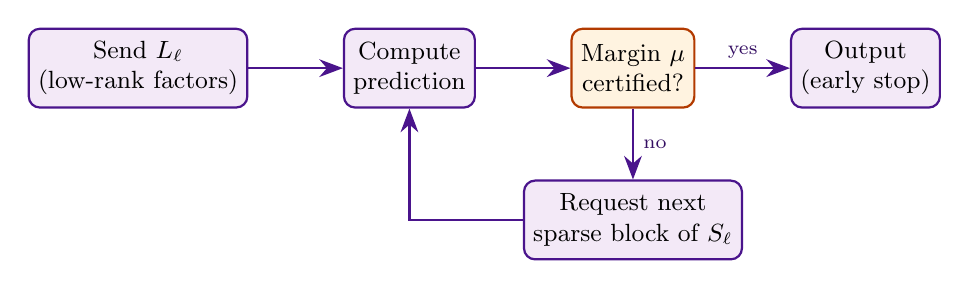
\begin{tikzpicture}[
  box/.style={draw=accent, fill=coolc, rounded corners, minimum height=1cm, align=center, thick, font=\small},
  dec/.style={draw=accent3, fill=warmc, rounded corners, minimum height=1cm, align=center, thick, font=\small},
  ar/.style={-{Stealth[length=3mm]}, thick, accent},
  lab/.style={font=\scriptsize, text=accent!70!black}
]
\node[box] (send) at (0,0) {Send $L_\ell$\\(low-rank factors)};
\node[box, right=1.2cm of send] (comp) {Compute\\prediction};
\node[dec, right=1.2cm of comp] (cert) {Margin $\mu$\\certified?};
\node[box, right=1.2cm of cert] (out) {Output\\(early stop)};
\node[box, below=0.9cm of cert] (ref) {Request next\\sparse block of $S_\ell$};
\draw[ar] (send) -- (comp);
\draw[ar] (comp) -- (cert);
\draw[ar] (cert) -- node[above,lab]{yes} (out);
\draw[ar] (cert) -- node[right,lab]{no} (ref);
\draw[ar] (ref) -| ($(comp.south)+(0,0)$);
\end{tikzpicture}
\end{center}

\subsection{The certified early-stop rule}
\label{sec:cert}
Let $F$ be the downstream map from the cut to the output, and suppose $F$ is $\kappa$-Lipschitz
(local Lipschitz constants are estimable per layer). If the current reconstruction
$\hat A_\ell = L_\ell + S_\ell^{(j)}$ (after $j$ residual blocks) satisfies
$\norm{A_\ell-\hat A_\ell}\le \eta_j$, then the output moves by at most $\kappa\eta_j$.

\begin{theorybox}
\textbf{Certified equivalence.} If the output margin on the coarse prediction exceeds the
worst-case perturbation, $\mu > \kappa\,\eta_j$, then the decision on $\hat A_\ell$ is
\emph{provably identical} to the decision on the full dense tensor $A_\ell$ --- no accuracy
loss, only earlier stopping. Communication then scales as
\[
\text{(factor size for } L_\ell) \;+\; O\!\big(k\log(N/k)\big) \quad\text{instead of } O(N),
\]
with $k$ the number of sparse blocks actually requested before certification.
\end{theorybox}

\begin{claim}[to be proved]
Under the $A=L+S+E$ model with $\norm{E_\ell}\le\varepsilon_0$ and a $\kappa$-Lipschitz
downstream map, the progressive protocol returns a decision identical to dense inference on
every input whose margin exceeds $\kappa(\varepsilon_0+\text{residual after } k \text{ blocks})$,
using expected communication $O(r\!\cdot\!\text{(mode size)} + \bar k\log(N/\bar k))$, where
$\bar k$ is the mean certified sparse budget over the input distribution.
\end{claim}

\subsection{Communication scaling --- the payoff}
For dense transmission, cost $=O(N)$. For LoSpar-CI, cost $=$ (factors) $+\,O(k\log(N/k))$.
When $A_\ell$ is genuinely low-rank-plus-sparse, $r$ and $k$ are tiny relative to $N$, so the
saving grows with ambient dimension --- exactly the ultra-high-dimensional regime where dense
transmission hurts most.

% ================================================================
\section{Application domains (why the \texorpdfstring{$A=L+S+E$}{A=L+S+E} premise holds)}

\begin{itemize}[leftmargin=1.5em,itemsep=2pt]
\item \term{Hyperspectral imagery --- the strongest case.} Low-rank$+$sparse (+ Gaussian
noise) is canonical here: LRTV~\cite{lrtv} \emph{literally} decomposes an HSI into low-rank
$+$ sparse noise $+$ Gaussian noise (i.e.\ $L+S+E$); low-rank recovery~\cite{hsi_lowrank} and
low-rank tensor recovery~\cite{hsi_tensor} are standard.
\item \term{Dynamic medical volumes.} Otazo et al.~\cite{otazo} decompose accelerated dynamic
MRI into low-rank $+$ sparse; CT sequences likewise~\cite{ct_ls}. \emph{Note:} these exploit
\emph{temporal} correlation --- for a single static volume the support is spatial
compressibility~\cite{sparsemri} rather than a named $L+S+E$ result.
\item \term{Whole-slide pathology images.} WSIs carry extreme spatial redundancy and are
highly compressible~\cite{wsi_natcomm}. \emph{Honest caveat:} no paper models a WSI literally
as $L+S+E$; the justification is high spatial redundancy (a strong $L$ term), so phrase the
premise as ``low-rank structure with sparse informative regions,'' validated empirically per
modality before relying on certified early-stop.
\end{itemize}

% ================================================================
\section{LoSpar-CI for LLMs: extending the FSU pipelined-inference poster}
\label{sec:llm}

The framework above was developed for ultra-high-dimensional \emph{inputs}. For LLMs, the
right object is the \emph{KV cache}, which grows every token. ``KV-cache compression'' says
\emph{what}; ``online/real-time'' says \emph{when}. The feasible design uses both offline
and online work, but assigns them different jobs: a fixed weight-side projection creates the
low-rank bulk, while a small input-dependent residual is extracted block-wise as old cache
entries leave an exact hot window.

\subsection{Why the obvious target (the inter-stage activation) is the wrong one}
During autoregressive \emph{decoding} only one token crosses each stage boundary per step,
so the transmitted activation is a single hidden vector of size $H$ ($\approx 6$\,KB for a
3B model). A lone vector has no low-rank structure to exploit, and the poster's
$\approx 34.5$\,ms/token communication is dominated by \emph{round-trip latency and framework
overhead}, not by transmission volume ($6$\,KB over $1$\,Gbps is $\sim0.05$\,ms). Compressing
that activation therefore cannot help decoding --- an honest non-starter worth stating
plainly. (During \emph{prefill} the activation is a genuine $(\text{seq}\times H)$ tensor, so
progressive low-rank transmission \emph{does} cut long-prompt prefill communication --- a
secondary win, not the main one.)

\subsection{Two routes, and why the hybrid is the feasible one}
The earlier draft implicitly used an \term{activation-side route}: compute full $K,V$, then
repeatedly decompose the growing cache as $K\approx AB^\top+S_K$. This is data-adaptive but
puts decomposition on the decoding path. ``Real-time'' must not mean an SVD every token; on
small head dimensions that overhead can exceed dense attention.

The \term{weight-side route} factorizes $W_K,W_V$ once, offline, so each token is born in a
small latent space. Palu~\cite{palu}, Eigen Attention~\cite{eigenattn}, and MLA/
MHA2MLA~\cite{deepseekv2,mha2mla} establish this route. It is LoRA-like in timing (fixed
factors used at runtime), but it compresses inference activations rather than representing a
trainable weight update.

\begin{claimbox}
\textbf{Revised LLM design:} use the weight-side route for the low-rank bulk $L$ and the
activation-side route only for a sparse innovation $S$. Keep a recent exact window. When a
full block ages out, compute its residual against the fixed latent reconstruction once, retain
only the largest blocks/entries, and discard the dense copy. There is no online SVD and no
decomposition of the accumulated cache.
\end{claimbox}

\subsection{The structural model and direct execution}
For an old block $B$,
\[
K_B \;\approx\; \hat K_B(z_B^K)+S_B^K,\qquad
V_B \;\approx\; \hat V_B(z_B^V)+S_B^V,\qquad
z_t^K=x_tU_K,\;z_t^V=x_tU_V .
\]
Attention uses the latent term and sparse correction directly; it must not reconstruct the old
dense block. This requires a fused kernel and a measured complexity crossover. Eigen Attention
already establishes low-rank-space attention, so direct execution alone is not novel.

\subsection{RoPE is a design constraint, not a footnote}
LLaMA applies RoPE after the key projection, so a generic low-rank basis cannot always be
absorbed into the query. The first prototype should preserve complete RoPE coordinate pairs,
following RAP~\cite{rap}. A higher-compression variant can decouple a small exact positional
key from the semantic latent, following MLA/MHA2MLA~\cite{deepseekv2,mha2mla}, using
calibration plus parameter-efficient tuning. Any reported speedup must include RoPE transforms;
Eigen Attention reports that RoPE overhead can erase its latency benefit on LLaMA models.

\subsection{Why it fits the poster's architecture}
The poster gives each device whole layers and the complete KV for those layers. Each stage can
therefore retain its exact hot window plus latent--sparse old cache locally. Remote per-layer KV
sharding is intentionally excluded: it would add a network round trip inside every attention
layer. Compression budgets and the layer partition are chosen jointly so the slowest stage,
not average work, is minimized.

\subsection{The certificate becomes a budget allocator, not a per-token loop}
A global logit certificate that recomputes downstream layers after every residual increment is
too expensive for the fast path. Instead, calibrate per-layer/head attention-output error
$\mathcal E_{\ell h}(r,k,b)$ offline and allocate rank, residual blocks, and bit-width under a
global quality budget. A strict next-token certificate remains a small diagnostic experiment,
not the primary runtime protocol. This trades a stronger theorem for a more credible speedup.

\subsection{Which poster problems it helps --- and which it does not}
\begin{center}
\renewcommand{\arraystretch}{1.3}
\small
\begin{tabular}{@{}p{4.5cm}p{1.7cm}p{6.3cm}@{}}
\toprule
\textbf{Poster problem} & \textbf{Helps?} & \textbf{Mechanism} \\
\midrule
Memory wall (its core problem) & \textbf{yes, directly} & Latent$+$sparse old KV shrinks the per-device footprint without online SVD. \\
Context-length limit (its \emph{next} wall) & \textbf{yes} & KV grows with conversation; compressing it pushes the wall out $\Rightarrow$ longer chats on the same 3 devices. \\
Layer partition / load balancing & \textbf{yes} & A smaller KV budget relaxes the 16/6/6 memory constraint $\Rightarrow$ rebalance (where it meets SparsePipe). \\
Long-prompt prefill communication & partly & Progressive low-rank transmission of the $(\text{seq}\times H)$ prefill activation. \\
Per-token decoding communication ($\sim$34.5\,ms) & \textbf{no} & That is round-trip latency, not size. \\
Raw per-token compute latency & regime-dependent & A fused latent kernel can help at long context; block aging and indexing can hurt at short context. \\
\bottomrule
\end{tabular}
\end{center}

\begin{claimbox}
For LLMs, LoSpar-CI becomes a \emph{RoPE-safe latent--residual KV method for the poster's
distributed pipeline}. Its primary claim is a better memory--quality frontier and longer
stationary context. Latency is claimed only beyond a measured crossover where fused latent
attention repays aging and indexing overhead.
\end{claimbox}

\subsection{Positioning versus existing KV compression}
Palu/Eigen Attention/MLA already cover weight-side low rank; RAP handles RoPE-aligned
reconstruction-free projection; OjaKV~\cite{ojakv} combines exact anchors with online subspace
adaptation; STAR-KV~\cite{starkv} adapts rank; LCA~\cite{lca} condenses context directly
inside an MLA latent; and JoLT~\cite{jolt} preserves a projected
residual. The defensible novelty hypothesis is therefore the \emph{combination of a fixed
RoPE-safe latent, sparse prompt-specific innovations, and joint heterogeneous stage placement
with stationary per-layer KV}. The decisive ablation compares joint placement with the same
compressor under the fixed 16/6/6 split.

\subsection{Experiment plan on the poster's cluster}
\begin{itemize}[leftmargin=1.5em,itemsep=1pt]
\item \term{Pre-study:} calibrate fixed projection factors; measure pre/post-RoPE spectra
and sparse residual concentration by layer/head. Stop if $2\times$ compression costs more than
one percentage point average task quality.
\item \term{Testbed:} the poster's 3$\times$ Jetson Orin Nano cluster~\cite{poster}; compare
the fixed 16/6/6 split with the joint planner under identical precision and power modes.
\item \term{Baselines:} dense CI-Inf; Palu, Eigen Attention, RAP, OjaKV, and STAR-KV;
KIVI~\cite{kivi}; and paging/offload where portable. The same compressor under a fixed
partition is the decisive ablation.
\item \term{Metrics:} KV bytes per token, admitted context length, TTFT, median and P95
token latency, throughput, energy, copy/migration traffic, and task quality.
\item \term{Performance target:} $1.5\times$ end-to-end throughput or $2$--$4\times$ longer
stationary context at matched quality. Treat short-context batch-1 as a negative control.
\end{itemize}

% ================================================================
\section{Scoped first paper}

\begin{claimbox}
Fix \emph{one} modality, \emph{one} decomposition, \emph{one} refinement rule, and a small
prototype --- establish the structural premise empirically before adding scheduling/RL.
\end{claimbox}

\begin{itemize}[leftmargin=1.5em,itemsep=2pt]
\item \term{Modality:} whole-slide images \emph{or} hyperspectral (hyperspectral gives the
cleanest $L+S+E$ justification; WSI gives the most compelling scale story).
\item \term{Decomposition:} Tensor-Train for $L$~\cite{tt}; block-support encoding for $S$.
\item \term{Refinement rule:} margin-based certified early stop (\S\ref{sec:cert}).
\item \term{Prototype:} a two- or three-device edge cluster (as in the poster~\cite{poster}).
\item \term{Metrics:} communication bytes vs.\ dense at \emph{certified} (zero) or bounded
accuracy loss; fraction of inputs stopping at the coarse stage; end-to-end latency;
per-layer $L{+}S$ energy (a cheap pre-study establishing where the premise holds).
\item \term{Baselines:} dense transmission; a fixed-rate low-rank-only transmission (no sparse
refinement); a token-compression method (SparseVLM~\cite{sparsevlm} / DTC-WSI~\cite{dtcwsi})
adapted to the setting.
\end{itemize}

\begin{riskbox}
The $A=L+S+E$ premise may hold only weakly for some layers/modalities, weakening certified
early-stop. Mitigate by measuring per-layer low-rank$+$sparse energy \emph{first} (a cheap
empirical study) and applying LoSpar-CI only where the spectrum justifies it, with dense
fallback elsewhere. Second risk: estimating a tight Lipschitz constant $\kappa$ --- use
local/empirical estimates and a conservative margin, accepting occasional extra refinement
rather than uncertified errors.
\end{riskbox}

% ================================================================
\begin{thebibliography}{99}
\small
% --- collaborative inference ---
\bibitem{hexgen} Y.~Jiang et al. \emph{HexGen: Generative Inference of Large Language Model over Heterogeneous Environment.} ICML 2024. arXiv:2311.11514.
\bibitem{jupiter} S.~Ye et al. \emph{Jupiter: Fast and Resource-Efficient Collaborative Inference of Generative LLMs on Edge Devices.} IEEE INFOCOM 2025. arXiv:2504.08242.
\bibitem{poster} H.~Zhou and X.~Zhang. \emph{Poster: Distributed Pipelined Collaborative Inference for LLMs on Edge Device Clusters.} ACM HotMobile 2026.
% --- low-rank + sparse foundations ---
\bibitem{rpca} E.~J.~Cand\`es, X.~Li, Y.~Ma, J.~Wright. \emph{Robust Principal Component Analysis?} J.~ACM 58(3):11, 2011. DOI 10.1145/1970392.1970395.
\bibitem{trpca_cvpr} C.~Lu, J.~Feng, Y.~Chen, W.~Liu, Z.~Lin, S.~Yan. \emph{Tensor Robust Principal Component Analysis: Exact Recovery of Corrupted Low-Rank Tensors via Convex Optimization.} CVPR 2016, pp.~5249--5257.
\bibitem{trpca_pami} C.~Lu et al. \emph{Tensor Robust Principal Component Analysis with a New Tensor Nuclear Norm.} IEEE TPAMI 42(4):925--938, 2020. arXiv:1804.03728.
\bibitem{kolda} T.~G.~Kolda, B.~W.~Bader. \emph{Tensor Decompositions and Applications.} SIAM Review 51(3):455--500, 2009. DOI 10.1137/07070111X.
\bibitem{tt} I.~V.~Oseledets. \emph{Tensor-Train Decomposition.} SIAM J.~Sci.~Comput. 33(5):2295--2317, 2011. DOI 10.1137/090752286.
\bibitem{losparse} Y.~Li et al. \emph{LoSparse: Structured Compression of Large Language Models based on Low-Rank and Sparse Approximation.} ICML 2023, PMLR 202:20336--20350. arXiv:2306.11222.
\bibitem{linformer} S.~Wang, B.~Z.~Li, M.~Khabsa, H.~Fang, H.~Ma. \emph{Linformer: Self-Attention with Linear Complexity.} arXiv:2006.04768, 2020.
% --- LLM KV cache (low-rank + sparse) ---
\bibitem{palu} J.~Chang et al. \emph{Palu: Compressing KV-Cache with Low-Rank Projection.} ICLR 2025. arXiv:2407.21118.
\bibitem{eigenattn} U.~Saxena, G.~Saha, S.~Choudhary, K.~Roy. \emph{Eigen Attention: Attention in Low-Rank Space for KV Cache Compression.} Findings of EMNLP 2024.
\bibitem{shadowkv} H.~Sun et al. \emph{ShadowKV: KV Cache in Shadows for High-Throughput Long-Context LLM Inference.} ICML 2025. arXiv:2410.21465.
\bibitem{deepseekv2} DeepSeek-AI. \emph{DeepSeek-V2: A Strong, Economical, and Efficient Mixture-of-Experts Language Model} (introduces Multi-head Latent Attention with low-rank KV compression). arXiv:2405.04434, 2024.
\bibitem{mha2mla} Y.~Ji et al. \emph{Towards Economical Inference: Enabling DeepSeek's Multi-Head Latent Attention in Any Transformer-based LLMs.} ACL 2025.
\bibitem{rap} J.~Xin et al. \emph{RAP: KV-Cache Compression via RoPE-Aligned Pruning.} arXiv:2602.02599, 2026.
\bibitem{ojakv} Y.~Zhu et al. \emph{OjaKV: Context-Aware Online Low-Rank KV Cache Compression.} Findings of ACL 2026.
\bibitem{starkv} P.~Bhatnagar et al. \emph{STAR-KV: Low-Rank KV Cache Compression via Soft Thresholding for Adaptive Rank Control.} arXiv:2606.08382, 2026.
\bibitem{lca} \emph{Latent-Condensed Transformer for Efficient Long Context Modeling.} ACL 2026.
\bibitem{jolt} R.~Krishnan, V.~Schulz. \emph{A JoLT for the KV Cache: Near-Lossless KV Cache Compression via Joint Tucker and JL-Residual Allocation for LLMs.} arXiv:2607.12550, 2026.
\bibitem{h2o} Z.~Zhang et al. \emph{H2O: Heavy-Hitter Oracle for Efficient Generative Inference of Large Language Models.} NeurIPS 2023. arXiv:2306.14048.
\bibitem{quest} J.~Tang et al. \emph{Quest: Query-Aware Sparsity for Efficient Long-Context LLM Inference.} ICML 2024. arXiv:2406.10774.
\bibitem{kivi} Z.~Liu et al. \emph{KIVI: A Tuning-Free Asymmetric 2bit Quantization for KV Cache.} ICML 2024. arXiv:2402.02750.
\bibitem{lexico} J.~Kim, J.~Park, J.~Cho, D.~Papailiopoulos. \emph{Lexico: Extreme KV Cache Compression via Sparse Coding over Universal Dictionaries.} ICML 2025. arXiv:2412.08890.
% --- token compression ---
\bibitem{dtcwsi} T.~Rahman, A.~Tarkhan, R.~Chellappa, A.~S.~Baras. \emph{DTC-WSI: Dynamic Token Compression for Whole-Slide Images.} MIDL 2026 (OpenReview yMkSDJc445).
\bibitem{sparsevlm} Y.~Zhang, C.-K.~Fan, J.~Ma et al. \emph{SparseVLM: Visual Token Sparsification for Efficient Vision-Language Model Inference.} ICML 2025. arXiv:2410.04417.
\bibitem{tome} D.~Bolya et al. \emph{Token Merging: Your ViT But Faster.} ICLR 2023 (Oral). arXiv:2210.09461.
\bibitem{fastv} L.~Chen et al. \emph{An Image is Worth 1/2 Tokens After Layer 2: Plug-and-Play Inference Acceleration for Large Vision-Language Models (FastV).} ECCV 2024. arXiv:2403.06764.
\bibitem{vocollama} X.~Ye et al. \emph{VoCo-LLaMA: Towards Vision Compression with Large Language Models.} CVPR 2025. arXiv:2406.12275.
\bibitem{prumerge} Y.~Shang et al. \emph{LLaVA-PruMerge: Adaptive Token Reduction for Efficient Large Multimodal Models.} ICCV 2025. arXiv:2403.15388.
% --- successive refinement / early exit ---
\bibitem{equitzcover} W.~H.~R.~Equitz, T.~M.~Cover. \emph{Successive Refinement of Information.} IEEE Trans.~Inf.~Theory 37(2):269--275, 1991. DOI 10.1109/18.75242.
\bibitem{jpeg} G.~K.~Wallace. \emph{The JPEG Still Picture Compression Standard.} IEEE Trans.~Consumer Electronics 38(1), 1992. DOI 10.1109/30.125072.
\bibitem{branchynet} S.~Teerapittayanon, B.~McDanel, H.~T.~Kung. \emph{BranchyNet: Fast Inference via Early Exiting from Deep Neural Networks.} ICPR 2016, pp.~2464--2469.
\bibitem{deebert} J.~Xin, R.~Tang, J.~Lee, Y.~Yu, J.~Lin. \emph{DeeBERT: Dynamic Early Exiting for Accelerating BERT Inference.} ACL 2020, pp.~2246--2251.
% --- compressed sensing ---
\bibitem{candestao} E.~J.~Cand\`es, T.~Tao. \emph{Near-Optimal Signal Recovery From Random Projections: Universal Encoding Strategies?} IEEE Trans.~Inf.~Theory 52(12):5406--5425, 2006.
\bibitem{donoho} D.~L.~Donoho. \emph{Compressed Sensing.} IEEE Trans.~Inf.~Theory 52(4):1289--1306, 2006.
% --- application-domain structure ---
\bibitem{lrtv} W.~He, H.~Zhang, L.~Zhang, H.~Shen. \emph{Total-Variation-Regularized Low-Rank Matrix Factorization for Hyperspectral Image Restoration.} IEEE TGRS 54(1):178--188, 2016.
\bibitem{hsi_lowrank} H.~Zhang, W.~He, L.~Zhang, H.~Shen, Q.~Yuan. \emph{Hyperspectral Image Restoration Using Low-Rank Matrix Recovery.} IEEE TGRS 52(8):4729--4743, 2014.
\bibitem{hsi_tensor} Y.~Fan et al. \emph{Hyperspectral Image Restoration Using Low-Rank Tensor Recovery.} IEEE JSTARS 10(10):4589--4604, 2017.
\bibitem{otazo} R.~Otazo, E.~Cand\`es, D.~K.~Sodickson. \emph{Low-rank plus sparse matrix decomposition for accelerated dynamic MRI with separation of background and dynamic components.} Magnetic Resonance in Medicine 73(3):1125--1136, 2015.
\bibitem{ct_ls} S.~Gou et al. \emph{CT Image Sequence Restoration Based on Sparse and Low-Rank Decomposition.} PLoS ONE 8(9):e72696, 2013.
\bibitem{sparsemri} M.~Lustig, D.~Donoho, J.~M.~Pauly. \emph{Sparse MRI: The Application of Compressed Sensing for Rapid MR Imaging.} Magnetic Resonance in Medicine 58(6):1182--1195, 2007.
\bibitem{wsi_natcomm} S.~Lee et al. \emph{Adaptive compression framework for giga-pixel whole slide images.} Nature Communications, 2025. DOI 10.1038/s41467-025-66889-0.
\end{thebibliography}

\end{document}
